\documentclass{article}
\usepackage{graphicx}
\usepackage[margin=1.5cm]{geometry}
\usepackage{amsmath}

\begin{document}

\title{Wednesday Reading Assessment: Unit 1, Electric Potential}
\author{Prof. Jordan C. Hanson}

\maketitle

\section{Memory Bank}

\begin{itemize}
\item $\vec{E} = -\frac{dV}{dx} \hat{x}$ ... One dimensional case
\item $\vec{E} = -\nabla V$ ... General case
\end{itemize}

\section{Electric Potential and Potential Energy}

\begin{enumerate}
\begin{figure}[ht]
\centering
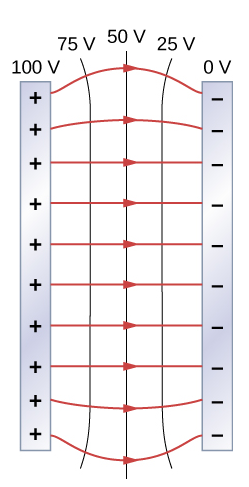
\includegraphics[width=0.15\textwidth]{plates.png}
\caption{\label{fig:hill} Voltage is a linear function of distance from the positive plate to the negative plate.}
\end{figure}
\item Consider Fig. \ref{fig:hill}.  Suppose the voltage is 100V at the positive plate.  What is the voltage half-way between the plates, if the E-field is constant and the voltage at the negative plate is 0V? \\ \vspace{1cm}
\item Consider Fig. \ref{fig:hill}.  Suppose the voltage is 100V at the positive plate.  What is the voltage \textit{two-thirds} of the way across, towards the negative plate? \\ \vspace{1cm}
\item If the distance between the plates is 5 mm, what is the E-field value?  (Remember, it is a constant in this case). \\ \vspace{1cm}
\item Draw a graph of the voltage versus position for Fig. \ref{fig:hill}. \\ \vspace{1cm}
\end{enumerate}

\end{document}
